% RELATED WORK
\section{Related Work \& Background}
\label{chapter:relatedwork}

In the literature, there are several algorithms focusing on path planning. In this section, existing research are introduced relevant to the context of this study where the motivation is to handle existence of multiple objectives and partial observability in path planning.

Bayili and Polat introduced a multi-objective path planning algorithm, Limited Damage A*  \cite{LDAStarBayili:2008} considering damage as a feasibility criterion in addition to distance. When an agent navigates in a threat zone, it is exposed to an additive damage. An upper bound is predefined for maximum damage that can be exposed and the algorithm discontinues the search on paths with damage score exceeding this threshold. The algorithm was shown to find suboptimal solutions with a reasonable time performance compared to MOA*. 

Tarapata presented multi-objective approaches to shortest path problems in his study \cite{Tarapata:2007}. He gave a classification of multi-objective shortest path (MOSP) problems and discussed different models of them. Also he presented methods of solving the formulated optimization problems. Analysis of the complexity of the presented methods and ways of adapting of classical algorithms for solving MOSP problems were described in detail. The comparison of the effectiveness of solving selected MOSP problems were defined as mathematical programming problems and multi-weighted graph problems. Experimental results of using the presented methods for multi-criteria path selection in a terrain-based grid network were given.

Guo et al. concentrated on the problem of multi-objective path planning (MOPP) for the ball and plate system in their study \cite{Guo:2009}. The goal of MOPP was to obtain the safe -without colliding with hazardous obstacles- and shortest path for the ball to follow. The environment was represented by distance and hazard map which represents possible collisions between the ball and the obstacles. They used an entropy-based method to calculate weights of objectives for each grid node. In simulation results, the path obtained by multi-objective method was much safer when compared to single-objective A* algorithm.

In \cite{Mitchell:2009}, Mitchell et al. examined the problem of planning a path through a low dimensional continuous state space subject to upper bounds on several additive cost metrics. For the single cost case, their previously published research has proposed constructing the paths by gradient descent on a local minimal free value function. This value function was the solution of the Eikonal partial differential equation, and efficient algorithms have been designed to compute it. In their paper, they proposed an auxiliary partial differential equation with which they evaluated multiple additive cost metrics for paths which are generated by value functions; solving this auxiliary equation adds little more work to the value function computation. They also proposed an algorithm which generates paths whose costs lie on the Pareto optimal surface for each possible destination locations, and a path can be chosen from those paths which satisfy the constraints. The procedure was practical when the sum of the state space dimension and the number of cost metrics is roughly six or less.

Evolutionary methods were also proposed for multi-objective path planning. A recent study by Pangilinan et al. \cite{Pangilinan} has introduced an evolutionary algorithm for multi-objective shortest path problem. They draw the picture of their 2-D static (stable obstacles and target) environment as a graph. Initial population was created by randomly generated individuals where each has a random ordered path from initial position to goal position. They used binary tournament selection for mating. Strength Pareto Evolutionary Algorithm (SPEA2) \cite{spea2:2001} was used to evaluate fitness values of individuals and to select them for survival. They defined density function of fitness evaluation to avoid from genetic drift. For genetic operators, they used one-point crossover and mutation. Their results show that their algorithm is a good alternative in finding a subset of efficient solutions for multi-objective shortest path problems when performance issues like complexity, diversity and non-dominal optimal solutions become obstructions.

Castillo et al. also worked on evolutionary algorithms for MOPP in their study \cite{Castillo:2007}. They defined a genetic off-line point-to-point agent path planner which tries to find valid paths. They concentrated on two constraints which are path length and difficulty (each path has a difficulty which is calculated from predefined weights) in their 2-D static grid environment. They compared their results with researches from 90's and obtain better results.

Bukhari et al. came up with an optimization technique for dynamic online path planning and optimization of the path \cite{Bukhari:2010}. It addresses the issues involved during path planning in dynamic and unknown environments cluttered with obstacles and objects. A simulated ant agent system is proposed using modified ant colony optimization algorithm for dealing with online path planning. It is compared with evolutionary techniques on randomly generated environments; with constraints like different obstacle ratio and grid sizes. The proposed algorithm generates and optimizes paths in complex and large environments with several constraints.

Nasrollahy et al. proposed a particle swarm optimization algorithm as a multi-agent search technique, for path planning in dynamic and known (fully observable) environments in order to minimize total path planning time while avoiding local optimums \cite{Nasrollahy:2009}. They created a small-scale model of search system moving goal position and obstacles. These obstacles were defined as circular shapes and agents get around of these obstacles. They tried to optimize global best path through the goal position. Although they mentioned about effectivity of proposed algorithm, they did not give concrete results and comparisons with other methods.

Dozier et al. gave a new selection method for multi objective path planning (MOPP) in \cite{Dozier:1998}. They introduced fuzzy tournament selection algorithm which combines fuzzy inference with tournament selection to select candidate solution paths. This selection was based on the euclidean distance from initial to goal position, the sum of the changes and the average change in the slope of a path.

Complete discussion of multi-objective evolutionary algorithms (MOEA) can be found in \cite{MOOUEA}. Also \cite{Coello:2000}, gives a summary of current approaches in MOEA and emphasizes the importance of new approaches in exploiting the capabilities of evolutionary algorithms in multi-objective optimization.

Algorithms on incremental search aim to generate an initial sub-optimal path, and try to improve it during the consequent iterations to make it closer to the optimal. Stentz et al. proposed the Dynamic A*, D* \cite{DStar:1994} which guarantees to be optimal and is functionally equivalent to re-planning from scratch. Later, D* Lite was proposed by Koenig et al. \cite{Koenig:2002} which utilized the same navigation strategy with D* but algorithmically different. It was based on Lifelong Planning A* (LPA*) \cite{LPAStarKoenig:2004}. D* Lite basically works as A* in the first iteration, then only updates for changed weights in environment. They prove that D* Lite was at least as efficient as D*.

\subsection{Multi Objective A* (MOA*)}

Classical A* \cite{AStarHart:1968} is a complete and optimal solution for the cases where only a single optimization criteria is crucial for path cost. On the other hand, real-world applications generally consider more than one criteria at the same time, which could not be converted, reduced or combined with each other. In this manner, multi objective A* (MOA*) \cite{MOAStewart:1991} extends classical A* to handle multiple objectives that inherently exist in many application domains. It uses the evaluation function $F(n) = G(n) + H(n)$ similar to A* but functions return vectors instead of scalar values. Size of the vector is the number of objectives to be optimized. If there is only one objective MOA* becomes standard A*. Like A*, it provides complete and optimal solutions when heuristic function is admissible which means the heuristic estimation of every objective is not overestimated.

MOA* keeps track of state expansions using {\it OPEN} (to be processed nodes) and {\it CLOSED} (already processed nodes) sets. Non-dominated states are maintained in a subset of {\it OPEN} named {\it ND} which is formed by the elements that are not dominated by any other element of this set and any of the discovered solutions.

At each iteration of the algorithm, first the best alternative node is selected from {\it ND}. Then, the selected node is checked whether it is in the set of goal nodes or not. If so, the current node and its path cost vector are added to the solution set and the iteration continues with selection of a new node. Otherwise, the adjacent nodes of current node are generated. At this step, for all generated adjacent nodes, the  newly generated node $n’$ is checked for being generated for the first time. If so, its path cost estimate vector $F(n’)$, traversed path cost vector $G(n’)$ and the heuristic estimate vector $H(n’)$ are computed, and the newly generated node is added to {\it OPEN} set. If the node is not explored for the first time, there is a possibility that a path passes through this node with non-dominated costs to other candidates. Then the node and its non-dominated cost vectors are taken into consideration in the following steps of the solution. The algorithm iterates over the above steps until the {\it ND} set becomes empty. Finally, solution paths are generated by following back-pointers from goal to start. 

%One of the important properties of this algorithm is the non-dominance property of the elements in the solution set over one another, which is also utilized in the {\it ND} set. This property ensures optimality, and for a set \Sigma containing elements of compatible vectors of same type, non-dominance can be formulated as: \[ \]

\subsection{D* Lite}

D* Lite \cite{Koenig:2002} is one the of most popular goal-directed autonomous agent navigation algorithms and widely used in unknown environment. It is an adaptation of Lifelong Planning A* \cite{LPAStarKoenig:2004} which is an incremental derivation of A* \cite{AStarHart:1968}. It determines the same paths as D* Algorithm \cite{DStar:1994} and moves the agent the same way but it is algorithmically different. Incremental search methods reuse information from previous searches to find solutions to similar problems much faster than is possible by solving each search task from scratch.

D* Lite Algorithm is a reverse or backward searching method where searching starts from the target position. It is able to re-plan from current position when a weight has been changed in the environment, i.e. there is a new obstacle blocking the path. It divides the environment into grids and path finding and agent's movement are from grid to grid.

\subsubsection{Overview}

Before considering an introduction to the problem that D* Lite covers, think about an agent path planning and navigation task in a dynamic unknown environment. In this scenario, agent always observes its current cell's neighbour cells and try to move one of them if it is traversable. Agent starts from start cell and moves through to the goal cell. It always try to compute the shortest (or minimized some other cost metric as determined by edge cost) path assuming that unexplored cells are traversable. Next, the agent try to follow found path until an untraversable cell is observed or reached to target cell successfully. Otherwise, the agent should recompute a shortest path from its current location to the target. Figure \ref{fig:dStarLiteExample}, simply represents the knowledge of cell states before and after of a movement. Each cell shows the goal distances from the agent's current cell to the goal. Known shortest path is drawn by an arrowed line. All of the cells in the grid except the adjacent of start cell are unexplored before the agent has moved and are assumed to be traversable; these cells are painted white. Cells are shaded gray in the lower grid maze whose goal distances have changed during discovery. The efficiency of D* Lite comes from replanning path just according to these changed cells.

\begin{figure}
\centering
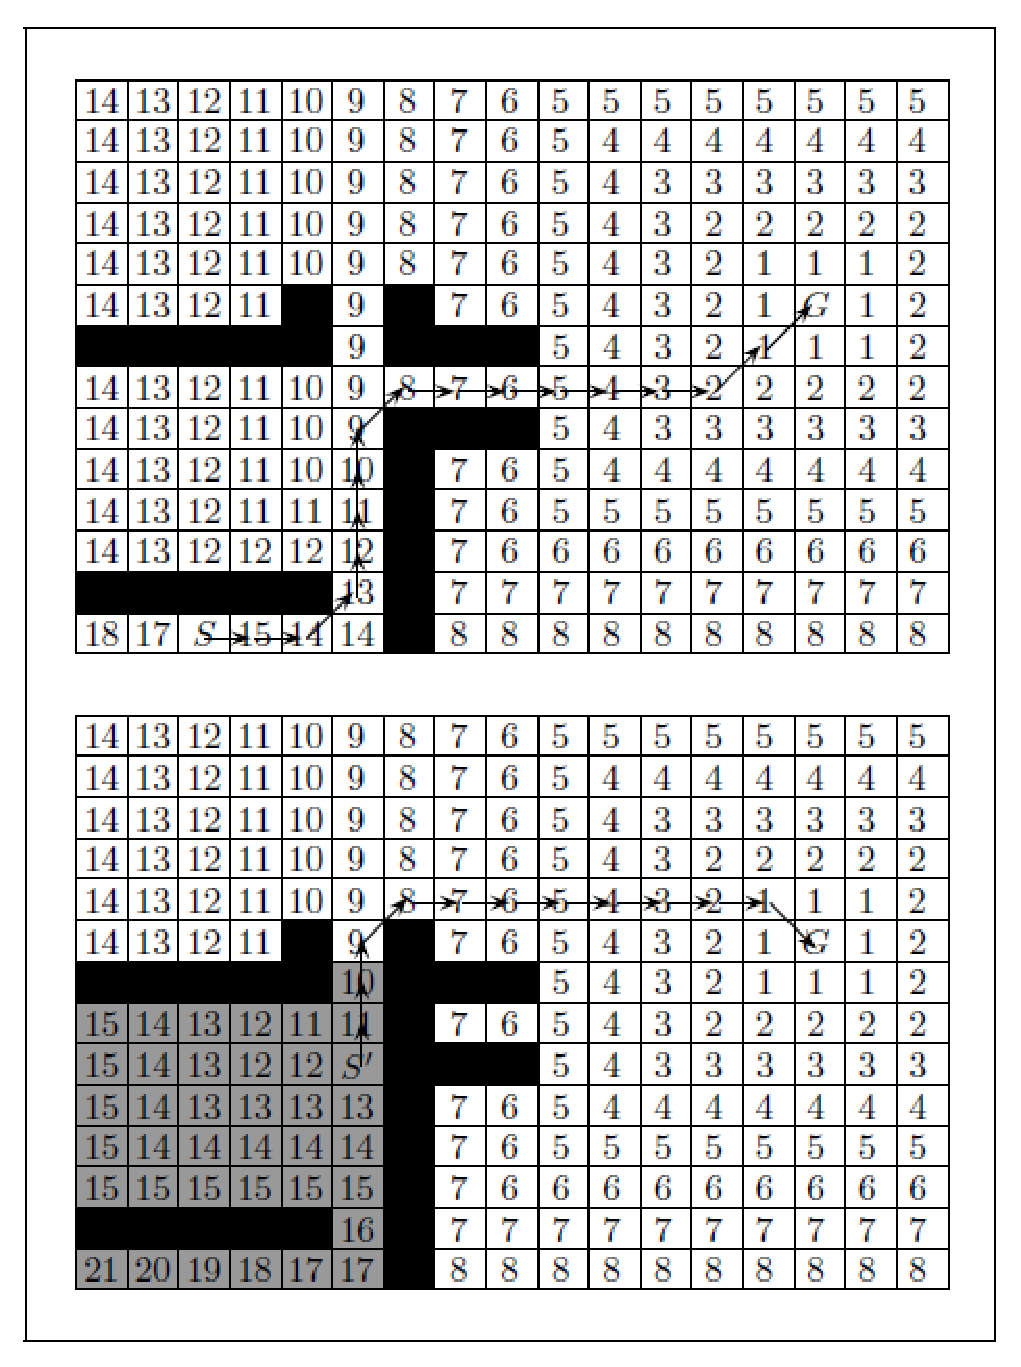
\includegraphics[width=2in]{dstarlite/dStarLiteExample}
\caption{A Simple Grid Search Representation}
\label{fig:dStarLiteExample}
\end{figure}

\subsubsection{Notation \& Formulation}
The notation is defined for D* Lite as follows: Let $S$ denotes the finite set of vertices of the graph. Let $Succ(s) \subseteq S$ and $Pred(s) \subseteq S$ denote the set of successors and predecessors of vertex $s \in S$, respectively. 

The cost of moving from vertex $s$ to $s' \in Succ(s)$ is denoted by $0 < c(s, s') \leq \infty$. D* Lite always gives shortest path found between $s_{start}$ and $s_{goal}$ where $s_{start}, s_{goal} \in S$. $g^*(s)$ is used to define the distance from $s_{start}$ to a vertex $s$. Heuristic function of D* Lite is also similar with classic A*, where $h(s_{goal}, s_{goal}) = 0$ and $h(s, s_{goal}) \leq c(s, s') + h(s', s_{goal})$; triangular inequality is held for all vertices $s \in S$ and $s' \in Succ(s)$ with $s \neq s_{goal}$.

D* Lite maintains an estimate $g(s)$ of the start distance $g^*(s)$ of each vertex $s$, analogous to the \textit{g-values} of an A* search. D* Lite carries them forward from search to search. D* Lite also maintains a second kind of estimate of the start distances; the \textit{rhs-values} are one step lookahead values based on the \textit{g-values} and thus potentially better informed than the \textit{g-values}. The \textit{rhs-values} should always satisfy the following equation;

\[ rhs(s) = \left\{ \begin{array}{cc}
0 & \mbox{if $s=s_{start}$};\\
min_{s' \in Pred(s)}(g(s') + c(s', s)) & \mbox{otherwise}.\end{array} \right. \] 

A vertex is stated as locally consistent if and only if its \textit{g-value} is equal to its \textit{rhs-value}, otherwise it is locally inconsistent. In the case that all vertices are locally consistent, the \textit{g-values} of all vertices are equal to their start distances, $g^*(s)$ namely. Actually, D* Lite does not try to make all vertices locally consistent after some edge costs have changed. It is not required to recompute start distances which have been computed before and have not been changed. Also, it uses admissible heuristic information in order to focus the planning phase and updates only the related \textit{g-values} which are relevant to the computation of a shortest path.

The D* Lite algorithm is complete; it always finds a shortest path if one exists or terminates. If $g(s_{goal}) = \infty$ after the search, then no path is constructed between $s_{start}$ and $s_{goal}$. Otherwise, one can trace a shortest path from $s_{start}$ to any vertex $s_{u}$ by, starting at vertex $s_{u}$, and always tracing back from the current vertex $s$ to any predecessor $s'$ of $s$ that minimizes $g(s') + c(s', s)$ until $s_{start}$ is reached. Notice that ties are broken arbitrarily.

\subsubsection{Core Components and Details}

Consistency of a vertex in the search graph could be considered in several conditions. A vertex $s$ is called \textit{locally consistent} iff $g(s) = rhs(s)$ and \textit{locally inconsistent} iff $g(s) \neq rhs(s)$. Local inconsistency refers to those whose \textit{g-values} need to be updated to become locally consistent. In the same manner, a locally inconsistent vertex is called \textit{locally overconsistent} iff $g(s) > rhs(s)$ and \textit{locally underconsistent} iff $g(s) < rhs(s)$. These consistency situations are used to manage vertices.

Like A*, D* Lite also maintains a priority queue with heuristic information such that the most promising vertices are expanded first. This queue contains only the locally inconsistent vertices which are selected sequentially to be expanded according to their key values $k(s)$, a vector of two components:
\begin{gather*}
k(s) = [k_{1}(s); k_{2}(s)] \\
k_{1}(s) = min(g(s), rhs(s) + h(s, s_{goal})) \\
k_{2}(s) = min(g(s), rhs(s))
\end{gather*}
The first component of the key $k_{1}(s)$ corresponds to $f(s) = g*(s) + h(s, s_{goal})$ which is the \textit{f-value} of A*, and the second component $k_{2}(s)$ corresponds to the \textit{g-value} of A*. Keys are compared (and maintained in the priority queue) in lexicographic order where $k(s) \leq k(s')$ iff either $k_{1}(s) < k_{1}(s')$ or $k_{1}(s) = k_{1}(s')$ and $k_{2}(s) \leq k_{2}(s')$.

Thus, the key with the smallest value is taken from the priority queue and expanded. The queue has several functionalities; where \textit{top()} returns the vertex with the smallest priority, \textit{topKey()} returns the key value of the vertex at the top or $[\infty, \infty]$ if the queue is empty. \textit{pop()} removes and returns the vertex with the smallest key and finally, the member functions \textit{remove()} and \textit{insert()} removes a vertex from and inserts a vertex into the queue, respectively.

\begin{algorithm}
	\caption{D* Lite Outline}
	\label{algDLite-1}
	%\begin{spacing}{0.5}
	{\fontsize{9}{9}\selectfont
    \begin{algorithmic}[1] % line numbering every line
      \Function{calculateKey}{s}
      	\State \Return $[min(g(s), rhs(s)) + h(s_{start},s) + k_{m} ; min(g(s), rhs(s))];$
      \EndFunction
   	  \Statex
      \Function{initialize()}{}
      	\State $U = \varnothing;$
      	\State $k_{m} = 0;$
      	\ForAll{$s \in S$}
     		\State $rhs(s) = g(s) = \infty;$
     	\EndFor
      	\State $rhs(s_{goal}) = 0;$
      	\State $U.insert(s_{goal}, calculateKey(s_{goal}));$
	  \EndFunction
	  \Statex
	  \Function{updateVertex}{u}
   	  	\If{$u \neq s_{goal}$}
   	  		\State $rhs(u) = min_{s' \in succ(u)}(c(u,s') + g(s'));$
   	  	\EndIf
   	  	\If{$u \in U$} U.remove(u); \EndIf
   	  	\If{$g(u) \neq rhs(u)$}
   	  		\State U.insert(u, calculateKey(u));
   	  	\EndIf
   	  \EndFunction
	  \Statex	  
  	  \Function{computeShortestPath()}{}
      	\While{$U.topKey() < calculateKey(s_{start})$ $||$ $rhs(s_{start}) \neq g(s_{start})$}
      		\State $k_{old} = U.topKey();$
      		\State $u = U.pop();$
    	  	\If{$k_{old} < calculateKey(u)$}
   		  		\State U.insert(u, calculateKey(u));
   		  	\ElsIf{$g(u) > rhs(u)$}
    	      	\State $g(u) = rhs(u);$
				\ForAll{$s \in pred(u)$} updateVertex(s) \EndFor
			\Else
				\State $g(u) = \infty;$
				\ForAll{$s \in pred(u) \cup u$} updateVertex(s); \EndFor
	   	  	\EndIf
      	\EndWhile  	  
  	  \EndFunction
    \end{algorithmic}}
    %\end{spacing}
\end{algorithm}

\begin{algorithm}
	\caption{Cont'd of D* Lite Outline}
	\label{algDLite-2}
	%\begin{spacing}{0.5}
	{\fontsize{9}{9}\selectfont
    \begin{algorithmic}[1] % line numbering every line
	  \Function{plan()}{}
	  	\State $s_{last} = s_{start}$
      	\State initialize();
      	\State computeShortestPath();
      	\While{$s_{start} \neq s_{goal}$}
			\If{$g(s_{start}) = \infty$} there is no known path \EndIf
			\State $s_{start} = argmin_{s' \in succ(s_{start})}(c(s_{start},s') + g(s'));$
			\State Move to $s_{start}$;
   	      	\State Scan the graph for changed edge costs;
    	      	\If{Any weight cost changed}
    	      		\State $k_{m} = k_{m} + h(s_{last}, s_{start}));$
      			  	\State $s_{last} = s_{start};$
    	      		\ForAll {directed edges (u,v) with changed edge costs}
    	      			\State Update the edge cost c(u,v);
    	      			\State updateVertex(u);
    	      		\EndFor
		      		\State computeShortestPath();
    	      	\EndIf
		\EndWhile
  	  \EndFunction
    \end{algorithmic}}
    %\end{spacing}
\end{algorithm}

The D* Lite algorithm is started by calling \textit{plan()} method in Algorithm \ref{algDLite-2}. It first calls \textit{initialize()} in Algorithm \ref{algDLite-1} at $\lbrace 3 \rbrace$ to start the search. \textit{initialize()} sets priority queue \textit{U} to an empty set, the heap reordering variable $k_{m}$ to zero, and the \textit{g} and \textit{rhs-values} of all vertices to infinity. Initially, $s_{start}$ is the only consistent vertex and is inserted into the empty priority queue with its calculated key $k(s_{start})$. \textit{calculateKey()} method is used to calculate the key of corresponding given vertex. Key formulation and generation is indicated above. This initialization guarantees that the first call to \textit{computeShortestPath()} at line $\lbrace 4 \rbrace$ in Algorithm \ref{algDLite-2} performs an A* search that it expands the same vertices as A* would, in exactly the same order.

After first execution of \textit{computeShortestPath()}, a loop is processed until reaching to $s_{goal}$. In each iteration, when $g(s_{goal})$ is observed as $\infty$, one can infer that there is no known path between $s_{start}$ and $s_{goal}$. If this is the case, the algorithm can be terminated. Else, next vertex to move is determined as new $s_{start}$ with the equation in line $\lbrace 7 \rbrace$ in Algorithm \ref{algDLite-2} where minimum cost adjacent of current $s_{start}$.

At this point, a change in the edge costs is waited in the environment at line $\lbrace 9 \rbrace$. If any edge costs have changed, the heap variable $k_{m}$ is cumulatively updated with heuristic function of last visited and $s_{start}$ vertices. Then; for all changed edge costs, new cost $c(s, s')$ is recalculated and \textit{updateVertex()} is called to recompute the \textit{rhs-values} and keys of the vertices potentially affected by the changed edge costs. In addition, if any of the vertices potentially affected have become locally consistent or inconsistent, their membership in the priority queue is adjusted. The $k_{m}$ variable is important because repeated reordering of priority queue $U$ is expensive since it often contains large number of vertices. By cumulatively adding heuristic value between last visited vertex and start, whenever new priorities are computed, the variable $k_{m}$ has to be added to key value's first components. In this way, the order of vertices in the priority queue is unaffected when the agent moves and the priority queue doesn't need to be reordered.

Finally, \textit{computeShortestPath()} is called which repeatedly expands locally inconsistent vertices according to their priorities. If top key of $U$, $k_{old}$ is smaller than calculated new key of corresponding vertex $u$, this vertex is inserted into queue. When it expands a locally overconsistent vertex $u$ at $\lbrace 22 \rbrace$ in Algorithm \ref{algDLite-1}, \textit{g-value} is set as \textit{rhs-value} to make $u$ locally consistent. When a locally underconsistent vertex $u$ is expanded in $\lbrace 25 \rbrace$, the \textit{g-value} of $u$ is set to infinity. This makes the corresponding vertex $u$ either locally consistent or overconsistent. If it was locally overconsistent, then changing of its \textit{g-value} can effect the local consistency of its neighbours, or successors. Otherwise, if $u$ was locally underconsistent, then changing of its \textit{g-value} can effect the local consistency of itself and its neighbours. As a result, \textit{computeShortestPath()} must \textit{updateVertex()} for all of the vertices potentially effected by the change in their \textit{g-values}. It modifies their \textit{rhs-values}, checking their consistency, and adding them to or removing them from the priority queue as appropriate in \textit{updateVertex()} method in lines $\lbrace 10 - 15 \rbrace$. The vertices are expanded by \textit{computeShortestPath()} until the key of the next vertex $s'$ to be expanded is no less than that of $s_{goal}$ or until $s_{goal}$ is locally consistent. This behaviour is similar with A* where expands vertices until it expands $s_{goal}$ at which point the \textit{g-value} of $s_{goal}$ is equal to its start distance and the \textit{f-value} of the node to expand next is no less than the \textit{f-value} of $s_{goal}$.

At the end of the algorithm execution, one can trace back a shortest path from $s_{start}$ to $s_{goal}$ by always transitioning from the current vertex $s$, starting at $s_{goal}$ , to any predecessor $s'$ that minimizes $g(s') + c(s',s)$, breaking ties arbitrarily, until $s_{start}$ is reached.